\documentclass{scrartcl}

\usepackage[utf8]{inputenc}
\usepackage[T1]{fontenc}
\usepackage{lmodern}
\usepackage{graphicx}
\usepackage[french]{babel}
\usepackage{geometry}

\geometry{
    paper=a4paper, % Paper size
    top=2.5cm, % Top margin
    bottom=2.5cm, % Bottom margin
    left=2.5cm, % Left margin
    right=2.4cm, % Right margin
    headheight=0.75cm, % Header height
    footskip=1.5cm, % Space from the bottom margin to the baseline of the footer
    headsep=0.75cm, % Space from the top margin to the baseline of the header
}

\usepackage{blindtext}
\usepackage{amsmath, amsfonts, amsthm, amssymb}
\usepackage{braket, nicefrac}
\usepackage{siunitx}
\usepackage{enumitem, multicol}
\usepackage{float}  % Use option [H] to force the placement of a figure
\usepackage{keystroke}
\usepackage{pgfplots}\usepgfplotslibrary{units}\pgfplotsset{compat=1.16}
\setcounter{tocdepth}{3}
\usepackage[none]{hyphenat}
\usepackage[font=small,skip=0pt]{caption}
\usepackage{wrapfig}
\usepackage{hyperref}
\usepackage{fancyhdr}
\usepackage{lastpage}
\usepackage{textcomp} % For ~ char
\usepackage{booktabs}
\usepackage{setspace}

\hypersetup{
    pdfauthor = {UMMISCO},
    pdftitle = {GamaSenseIt - Manuel utilisateur},
    pdfsubject = {GamaSenseIt},
    pdfkeywords = {Capteur, UMMISCO, IRD, GamaSenseIt, QameleO},
    pdfstartview = {FitH},
    colorlinks = true,
    allcolors = darkgray,
    breaklinks = true
}

\pagestyle{fancy}
\fancyhf{}
\lhead{GamaSenseIt - Manuel utilisateur}
\chead{
\href{https://www.ummisco.fr}{
\includegraphics[height=16px]{resources/ummisco.png}}
\href{https://www.ird.fr}{
\includegraphics[height=16px]{resources/ird.png}}
}
\rhead{UMMISCO \textcopyright}
\cfoot{Page~\thepage~sur~\pageref*{LastPage}}

%------------------------------- Glossary --------------

\usepackage[xindy, toc, nogroupskip, nopostdot, nonumberlist, style=list, acronym]{glossaries}

\usepackage{glossaries-extra}
\renewcommand*{\glstextformat}[1]{\textit{#1}} % customize link color here

\makenoidxglossaries

%--------------------% Storage Path for images %-----------------%

\graphicspath{{graphics/}{Graphics/}{./}}

\begin{document}

    
\begin{titlepage}
    \centering


    \vspace{10cm}
    {\huge\bfseries Manuel utilisateur\par}
    \vspace{1cm}
    {\scshape\LARGE GamaSenseIt \par}

    \vspace{2cm}

    \begin{figure}[H]
        \begin{center}
            \href{https://www.ird.fr}{
\includegraphics[width=4cm]{resources/ird}}
            \hspace{0.5cm}
            \href{https://www.ummisco.fr}{
\includegraphics[width=7cm]{resources/ummisco}}
        \end{center}\label{fig:garde}
    \end{figure}

    \vspace{2cm}

    {\scshape\Large\bfseries Institut de recherche pour le développement\par}
    \vspace{1cm}
    {\scshape\bfseries Unité Mixte de Modélisation mathématique et informatique de systèmes complexes, naturels, biologiques ou sociaux\par}

    \vfill

    \large Juillet 2022

\end{titlepage}


    \clearpage
    \begin{spacing}{1.25} % Permet de réduire l'espace
        \tableofcontents
    \end{spacing}

    \section{Page d'acceuil}\label{sec:page-d'acceuil}

    blabla
    \section{Carte de capteurs}\label{sec:carte-de-capteurs}

    \begin{figure}[H]
        \begin{center}
            
\includegraphics[width=12cm]{resources/map}
        \end{center}
        \caption{Carte de capteurs}
        \label{fig:carte-de-capteurs}
    \end{figure}

    En cliquant sur ``Carte des capteurs'' depuis la page d'accueil ou ``Carte'' dans le menu à gauche,
    vous pourrez accéder à cette page comportant une carte avec la position des capteurs.
    Chaque capteur est indiqué à l'aide d'un petit marquer.
    Il sera de couleur verte s'il a emit depuis moins d'une heure, orange s'il a été actif les dernières 24h
    et rouge si cela fait plus d'un jour qu'aucune valeur n'est émise.
    Vous pouvez aussi avoir un aperçu du capteur en le survolant avec la souris.
    Cela affichera la photo, le nom et le temps écoulé depuis la dernière émission.
    Si vous cliquez sur celui-ci, vous serez alors redirigé vers la page du capteur en question.
    \section{Liste de capteurs}\label{sec:liste-de-capteurs}

    \begin{figure}[H]
        \begin{center}
            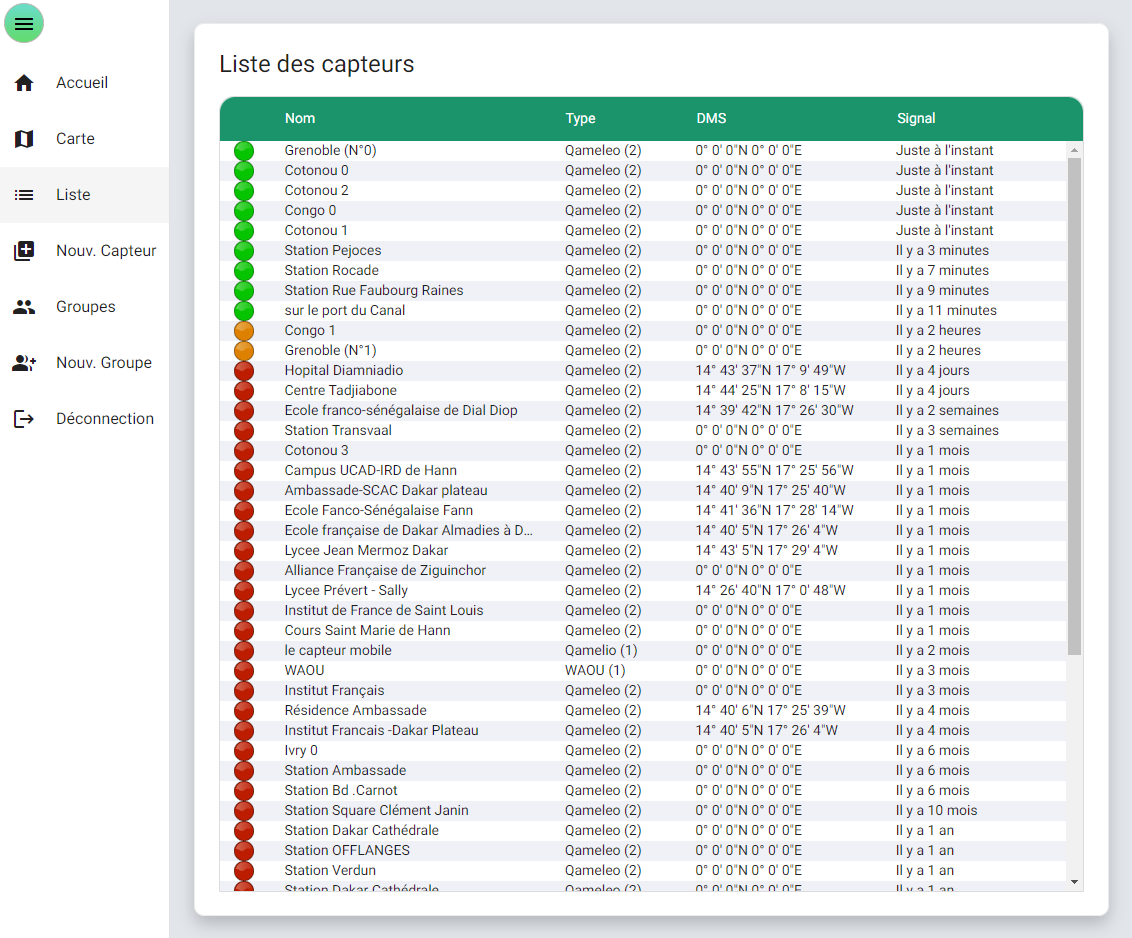
\includegraphics[width=12cm]{resources/list}
        \end{center}
        \caption{Liste de capteurs}\label{fig:liste-de-capteurs}
    \end{figure}

    En cliquant sur ``Liste des capteurs'' depuis la page d'accueil ou ``Liste'' dans le menu à gauche,
    vous pourrez visionner la liste de capteurs à votre disposition.
    Les capteurs sont triés par ordre de dernière émission de données.
    Chaque ligne comporte 5 indications : un voyant indiquant la dernière émission (vert pour moins d'une 1 h,
    orange pour moins de 24h et rouge pour plus d'un jour) puis vous avez le nom du capteur,
    le nom du modèle de capteur, sa position en DMS (degré minute seconde)
    et le temps depuis la dernière réception de données.
    Chaque ligne peut être cliquer pour afficher la page du capteur.

    \section{Page de capteur}\label{sec:page-de-capteur}

    \begin{figure}[H]
        \begin{center}
            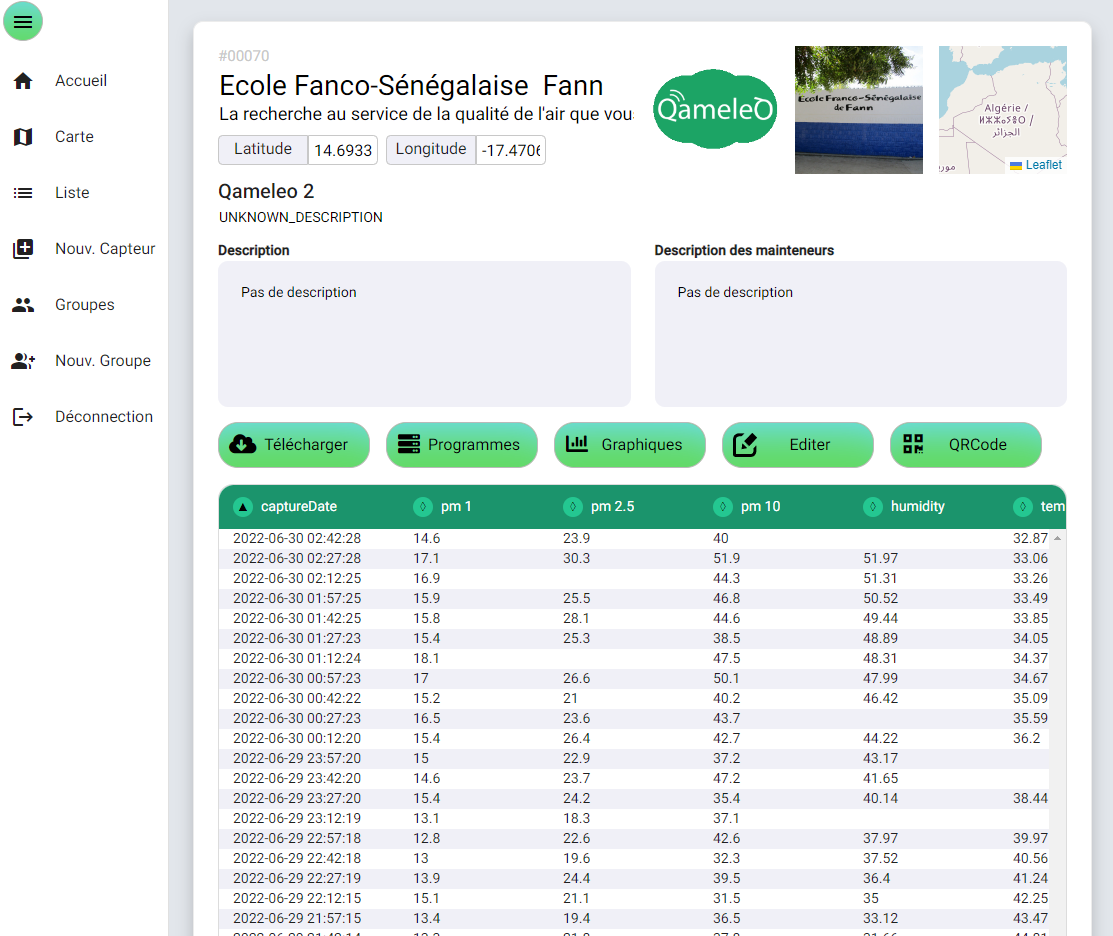
\includegraphics[width=12cm]{resources/sensor}
        \end{center}
        \caption{Page de capteur}
        \label{fig:page-de-capteur}
    \end{figure}

    Ceci est la page de présentation du capteur, elle permet de nombreuses actions :
    téléchargement des données, téléversement du programme, visualisation de graphique,
    éditions des informations du capteur et création de QRcode.
    En plus de cela elle permet d'écrire deux descriptions :
    une à destination des visiteurs et une autre pour les mainteneurs du capteur.
    Vous pouvez aussi observer les dernièrse données reçues via un tableau.
    \section{Téléchargement des données}\label{sec:telechargement-des-donnes}

    \subsection{Généralité}\label{subsec:generalite}

    \begin{figure}[H]
        \begin{center}
            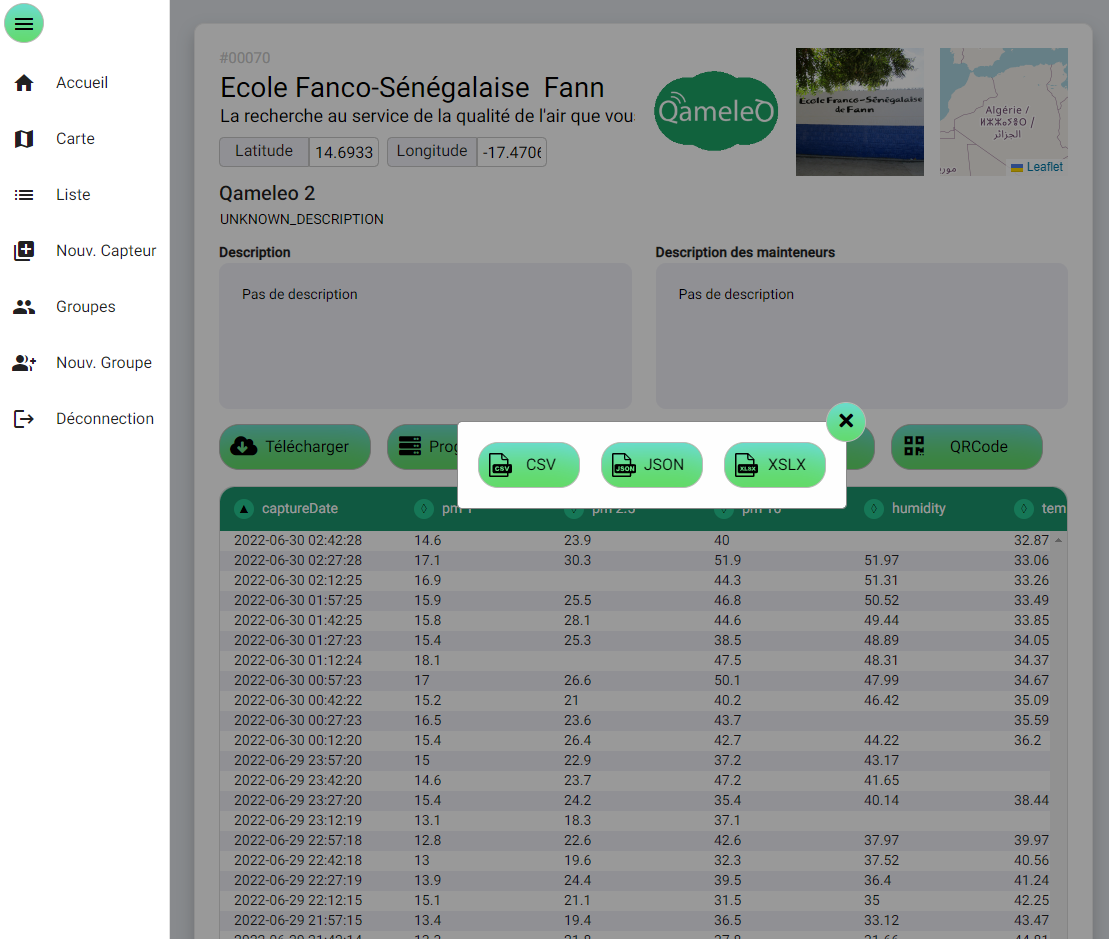
\includegraphics[width=12cm]{resources/sensor_download}
        \end{center}
        \caption{Téléchargement des données}\label{fig:telechargement-des-donnes}
    \end{figure}

    Après avoir appuyé sur ``Télécharger'' sur la page d'un capteur, une petite fenêtre
    s'ouvre vous demandant de choisir entre 3 formats, le format CSV, JSON et XSLX (Excel).
    Les formats CSV et JSON sont compressé via une archive ZIP pour permettre de les télécharger plus vite.

    \subsection{Format CSV}\label{subsec:csv}

    \begin{figure}[H]
        
\includegraphics[width=13cm]{resources/csv}
        \label{fig:csv}
    \end{figure}

    Le format csv possède 3 headers qu'il faudra ignorer : les noms, les identifiants, et les unités.
    Il faudra donc ignorer les 3 premières lignes.

    \begin{figure}[H]
        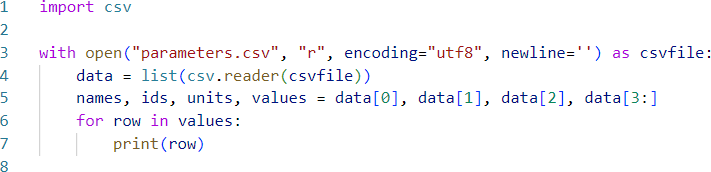
\includegraphics[width=11cm]{resources/csv_exemple}
        \caption{Script d'analyse de CSV}\label{fig:csv-exemple}
    \end{figure}

    Vous pouvez utiliser le script ci-dessus pour traiters les fichier CSV.

    \subsection{Format JSON}\label{subsec:json}

    \begin{figure}[H]
        
\includegraphics[width=13cm]{resources/json}
        \label{fig:json}
    \end{figure}

    Le format json est plus complet que le format CSV,  il contient en plus des informations sur le capteur et d'autres données.

    \begin{figure}[H]
        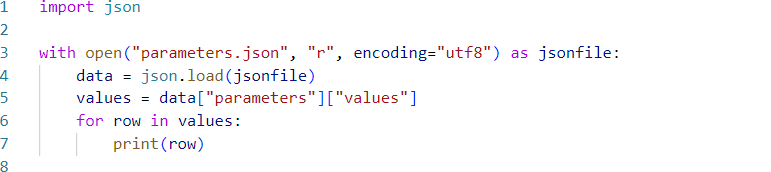
\includegraphics[width=11cm]{resources/json_exemple}
        \caption{Script d'analyse de JSON}\label{fig:json-exemple}
    \end{figure}

    Le script ci-dessus vous permettra le traitement des fichiers JSON.

    \subsection{Format XSLX}\label{subsec:xslx}

    \begin{figure}[H]
        \begin{center}
            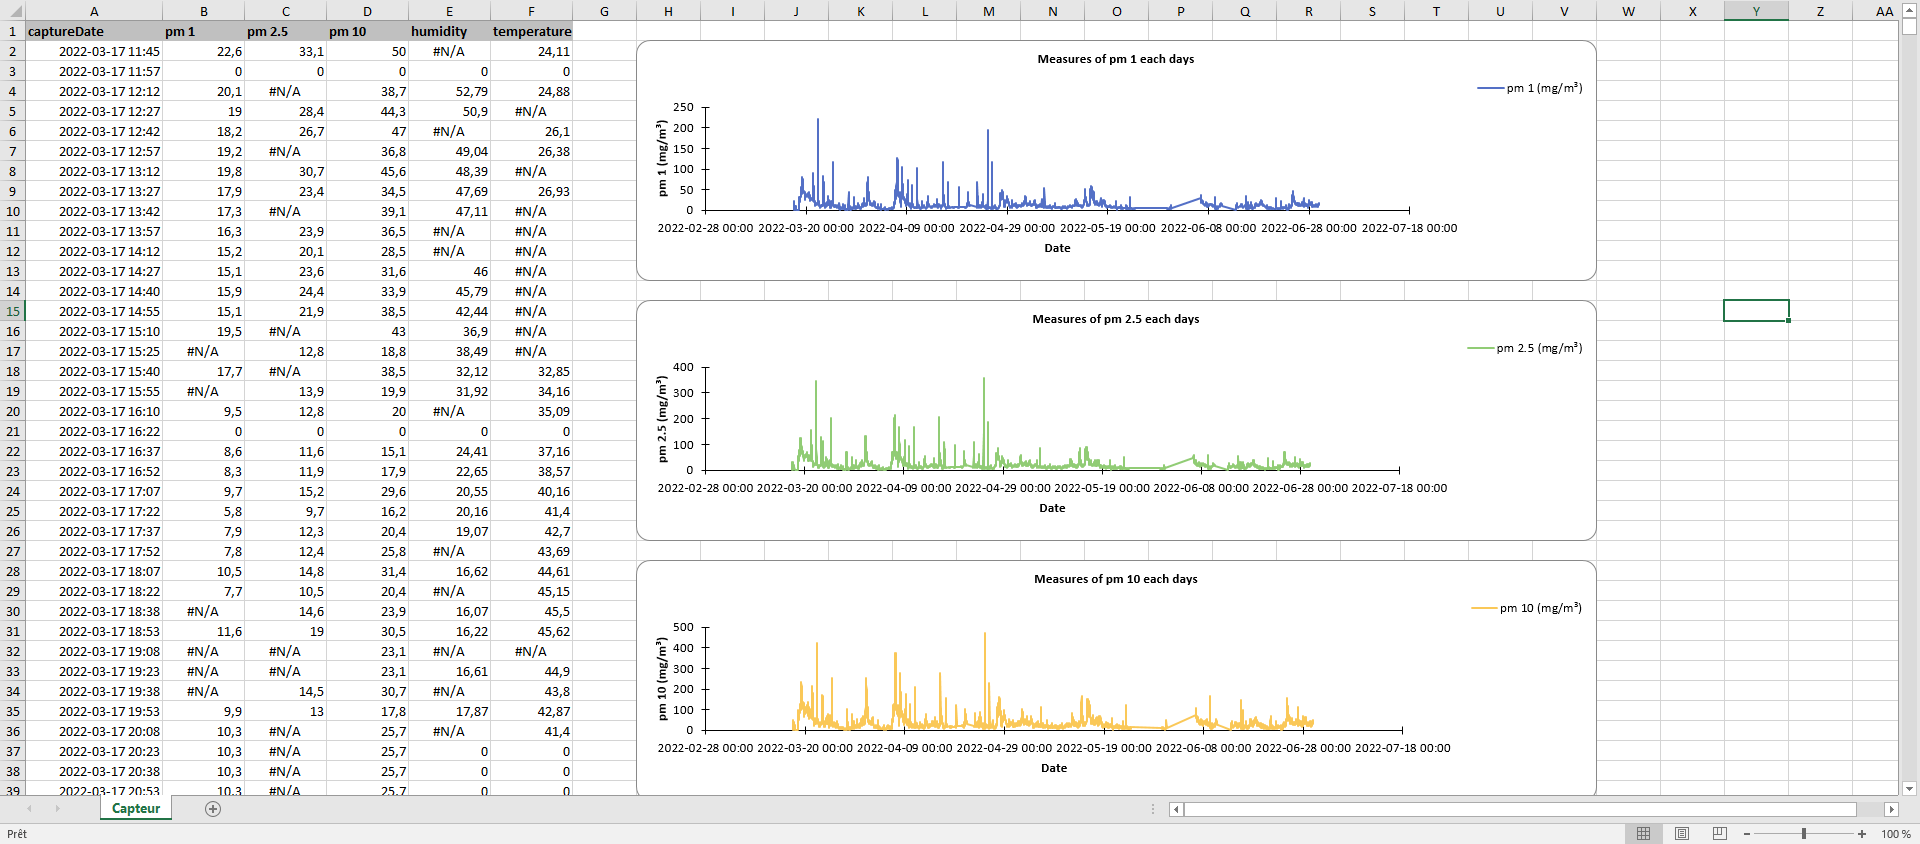
\includegraphics[width=14cm]{resources/xslx}
        \end{center}\label{fig:xslx}
    \end{figure}

    Le format XSLX est le format de fichier du logiciel Microsoft Excel.
    Vous aurez besoin de ce logiciel pour pouvoir ouvrir ce fichier.
    De plus, ce format comporte des courbes de données par défaut.

    \clearpage

    \section{Application de téléversement}\label{sec:application-de-téléversement}

    \subsection{Prérequis et Intallation}\label{subsec:prerequis-et-intallation}

        \begin{figure}[H]
            \begin{center}
                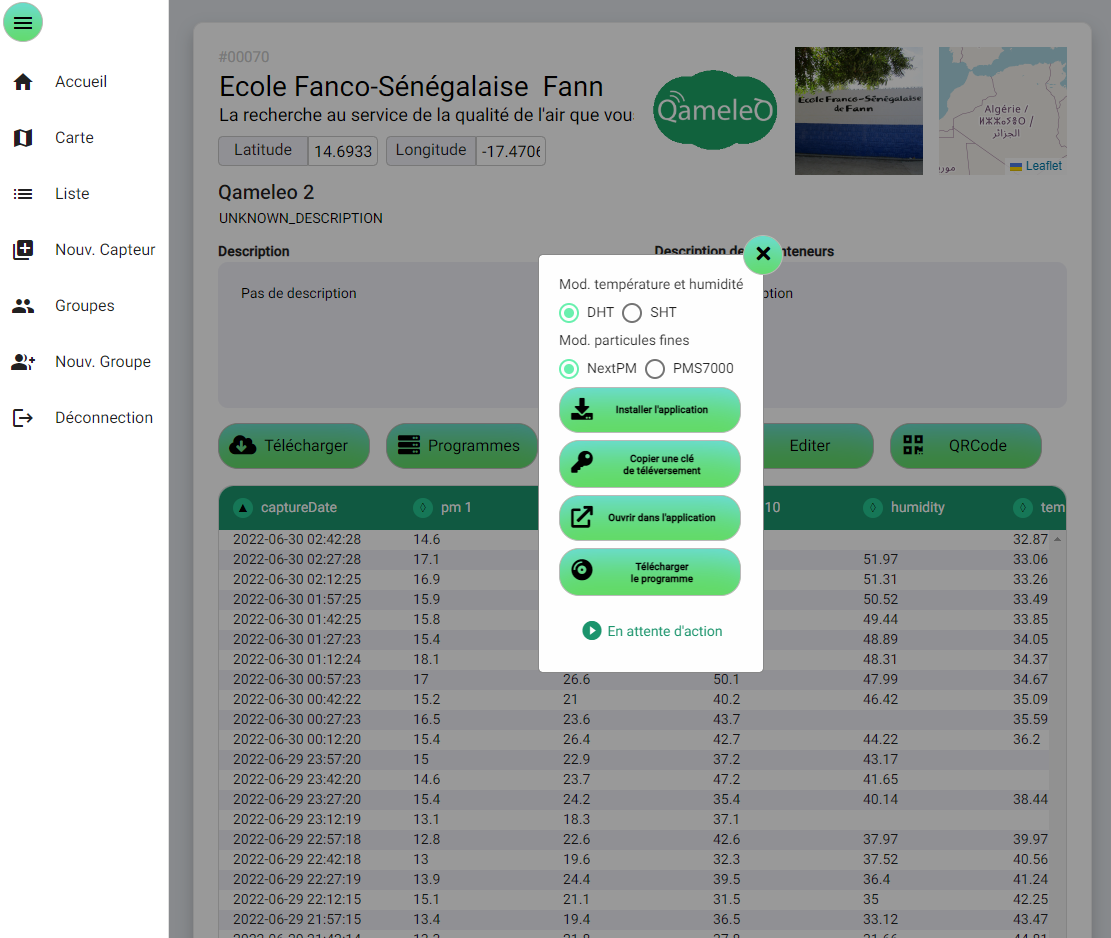
\includegraphics[width=12cm]{resources/sensor_app}
            \end{center}
            \caption{Page de l'application}\label{fig:page-de-l-application}
        \end{figure}

        Afin de permettre l'interaction entre le site web et l'Arduino, une application de bureau a été développée.
        Cette application est récupérable à partir de n'importe quel capteur en appuyant sur ``Programmes'' puis ``Installer l'application''.
        Vous récupérez alors une JAR, un programme utilisant java pour fonctionner.
        Si vous n'avez pas java installer, merci de suivre les indications sur \href{https://www.java.com}{www.java.com}.
        Une fois que vous lancez l'application, vous aurez un avertissement vous demandant une ``installation privilégié''
        si vous souhaitez utiliser pleinement les fonctionnalités fournies par windows (Ouverture de fichier et lancement de l'application depuis un navigateur).
        Suite à cela l'installation sera terminée.
        À noter qu'elle vous sera automatiquement redemandée si vous déplacer l'application.

    \subsection{Utilisation}\label{subsec:utilisation}

        \begin{figure}[H]
            \begin{center}
                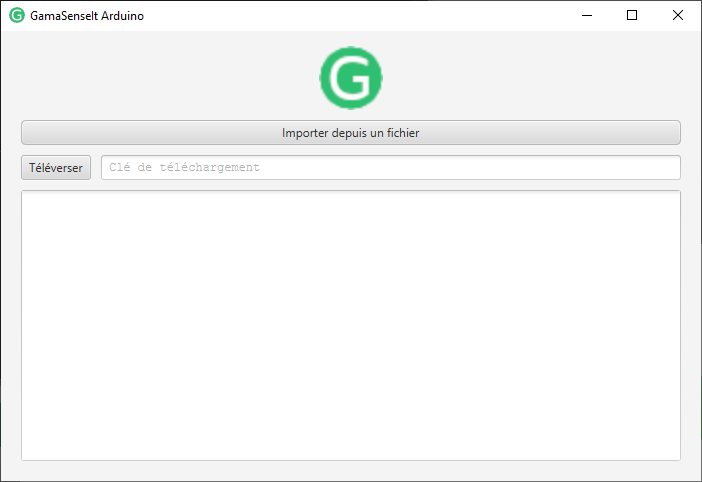
\includegraphics[width=12cm]{resources/app}
            \end{center}
            \caption{Application de téléversement}\label{fig:app-televersement}
        \end{figure}

        Sur cette application vous aurez 3 possibilités pour téléverser le programme d'un capteur :

        \begin{itemize}
            \item Via une clé de téléchargement
            \item En l'ouvrant depuis le navigateur (Windows seulement)
            \item En téléchargent le fichier (Windows et partiellement sur les autres)
        \end{itemize}

        \subsubsection{Téléversement par clé}

            Vous pouvez utiliser une clé que vous récupérer en cliquant sur ``copier une clé de téléversement''.
            Cette clé est alors valide pendant 15 min.
            Suite à cela, copier la clé dans le champ ``Clé de téléchargement'' puis appuyez sur ``Téléverser''.
            Il vous sera demandé de confirmer le télécharmeent et optionnellement, si le site ne support pas le https,
            de téléchargement de façons non sécurisé.

        \subsubsection{Téléversement par navigateur}

            Si vous êtes sur windows et avez suivi les étapes précédents vous pouvez appuier sur ``Ouvrir dans l'application''
            sur le site web puis confirmé sur l'application telle que précédament.

        \subsubsection{Téléversement par fichier}

            Pour procédé au téléversement en passant par un fichier, il faut tout d'abors télécharger le fichier
            en appuyant sur Télécharger le programme puis en sélectionnant la destination.
            Une fois ceci faites-vous pouvez directement ouvrir le fichier en cliquant dessus si l'application
            et correctement installer et que vous êtes sur une machine Windows.
            Dans le cas contraire vous pouvez ouvrir l'application puis appuyée sur ``Importer depuis un fichier'',
            puis sélectionner votre fichier et confirmer.

        \subsection{Moniteur Serial}\label{subsec:moniteur-serial}

            De plus l'application possède un moniteur serial permettant de voir les sorties du programme en temps réel.

    \section{Graphique de données}\label{sec:graphique-de-donnees}

    \begin{figure}[H]
        \begin{center}
            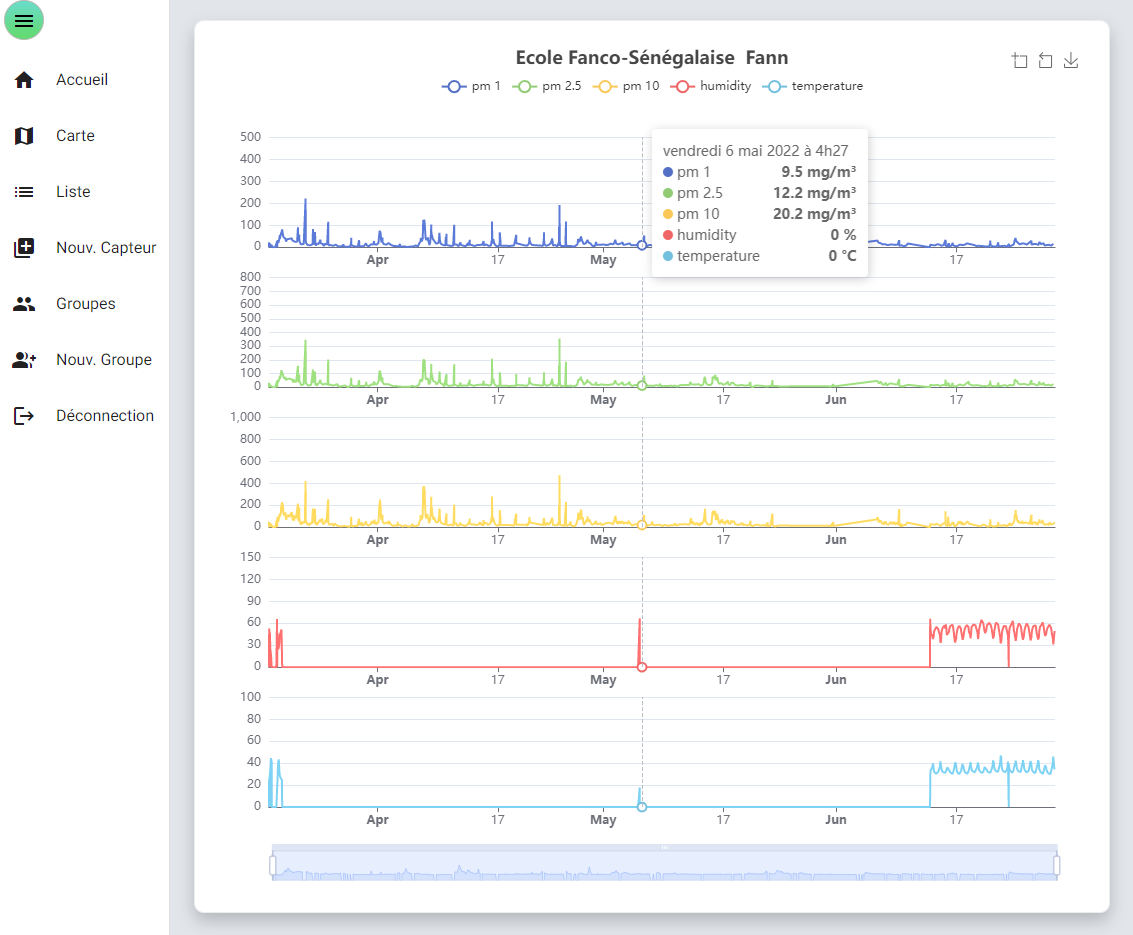
\includegraphics[width=12cm]{resources/graph}
        \end{center}
        \caption{Graphique de données}\label{fig:graphique-de-donnes)}
    \end{figure}

    Vous pouvez accéder à cette page depuis une page de capteur en appuyant sur ``Graphiques''.
    Une fois sur cette page, vous pouvez sélectionner une zone en l'agrandissant via la molette de votre souris.
    Vous pouvez aussi utiliser le sélecteur en bas de page.
    En passant votre souris à un point du graphique vous pourrez visionner l'ensemble des valeurs à l'instant choisi.
    En plus de cela, en haut à droit vous pouvez télécharger l'image actuellement afficher.
    \section{Edition des informations du capteur}\label{sec:edition des informations du capteur}


    \begin{figure}[H]
        \begin{center}
            
\includegraphics[width=12cm]{resources/edit}
        \end{center}
        \caption{Mode Edition de capteur}\label{fig:edition}
    \end{figure}

    Vous pouvez éditer le capteur en appuyant sur ``Editer''.
    Suite à cela vous pourrez modifier exclusivement le nom, l'indication, la description,
    la description des mainteneurs et la photo en cliquant sur celle-ci.
    \section{QR code}\label{sec:qr-code}

    \begin{figure}[H]
        \begin{center}
            
\includegraphics[width=5cm]{resources/qr_code}
        \end{center}
        \caption{QR Code}\label{fig:qr-code}
    \end{figure}

    En appuyant sur ``QRCode'' depuis la page d'un capteur vous pourrez télécharger le qrcode correspondant à la page.

    \section{Enregister un capteur}\label{sec:enregistrer-un-capteur}

    \begin{figure}[H]
        \begin{center}
            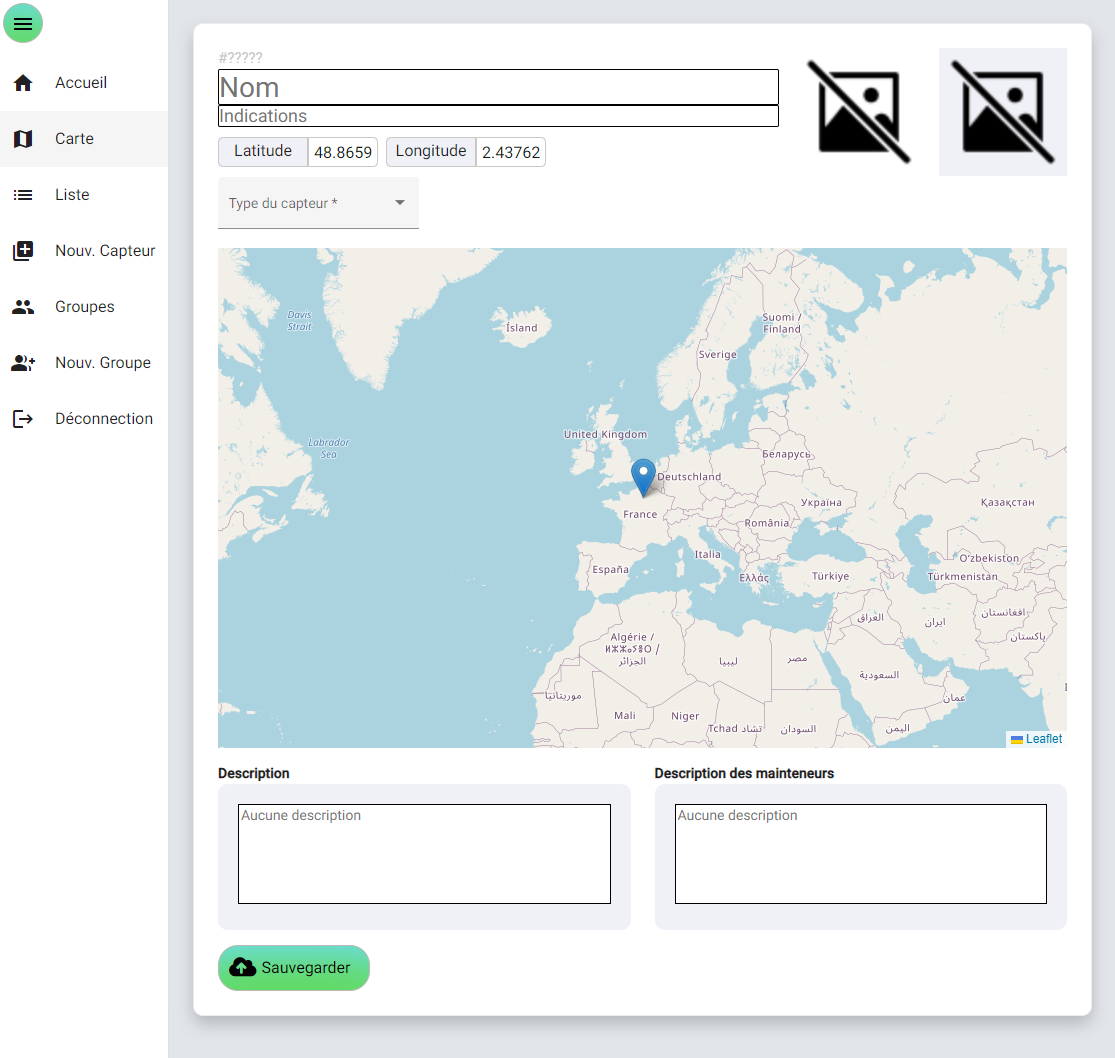
\includegraphics[width=12cm]{resources/create_sensor}
        \end{center}
        \caption{Page de création de capteur}\label{fig:create-sensor}
    \end{figure}

    Pour créer un capteur, vous devez être connecté.
    Après votre connexion vous devrez vous rendre sur ``Nouv. Capteur'' dans le menu.
    Une fois ceci, fais, il vous faut remplir le nom, les indications, l'image, le type du capteur,
    sélectionner l'aide de la carte l'emplacement du cpateur.
    Attention, vous ne pourrez plus changer la position de votre capteur,
    il faudra en recrée un si vous souhaiter le déplacer.
    Vous pouvez aussi ajouter une description à destination des visiteurs ou des mainteaneurs.

    Une fois les informations complété, vous pourrez sauvegarder le capteur et serez directement rediriger vers la page nouvellement créée.

    \clearpage
    \section{Les groupes}\label{sec:cree-un-groupe-d-utilisateurs-et-de-capteurs}

    \subsection{Fontionnement des groupes}\label{subsec:fontionnement-des-groupes}

        Pour permettre l'accès aux capteurs et leurs modifications des groupes ont été implémenter dans le logiciel.
        Il fonctionne de la manière suivante :
        Vous pouvez créé un groupe social permettant d'ajouter des membres et des capteurs en lecture seule.
        Dans ce groupe vous pouvez nommer un responsable et ainsi lui permettre de gérer le groupe.
        Vous pouvez créé un groupe de maintenance permettant d'ajouter capteurs et des membres qui pourront modifier ces capteurs
        et accéder à des informations permettant la mise en place et la maintenance des capteurs.
        Dans ce groupe vous pourrez nommer un responsable qui pourra ajouter ou supprimer des membres ainsi que des capteurs.
        Attention, ajouter un responsable lui permettra d'ajouter tous les capteurs du groupe à un groupe qu'il créera lui-même
        et sur lequel vous n'aurez aucun pouvoir.

        \begin{figure}[H]
            \begin{center}
                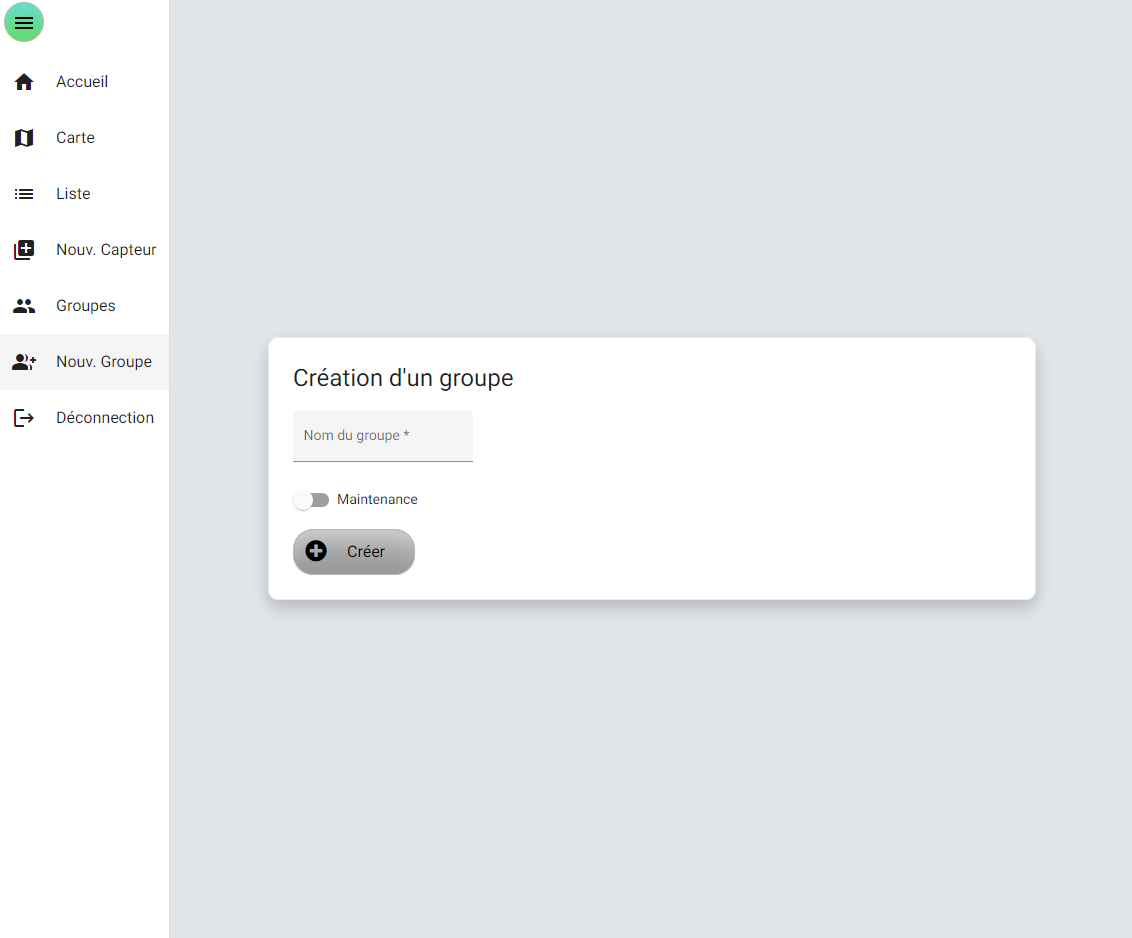
\includegraphics[width=12cm]{resources/create_group}
            \end{center}
            \caption{Page de création de groupe}\label{fig:create-group}
        \end{figure}

    \subsection{Créer un groupe}\label{subsec:creer-un-groupe}

        Pour créer un groupe vous devez être connecté, puis aller dans ``Nouv. Groupe''.
        Une fois ceci fait, vous devrez remplir le nom puis choisir si le groupe est de maintenance ou non.
        Pour terminer appuyer sur créer.

    \subsection{Rechercher un groupe}\label{subsec:rechercher-un-groupe}

        \begin{figure}[H]
            \begin{center}
                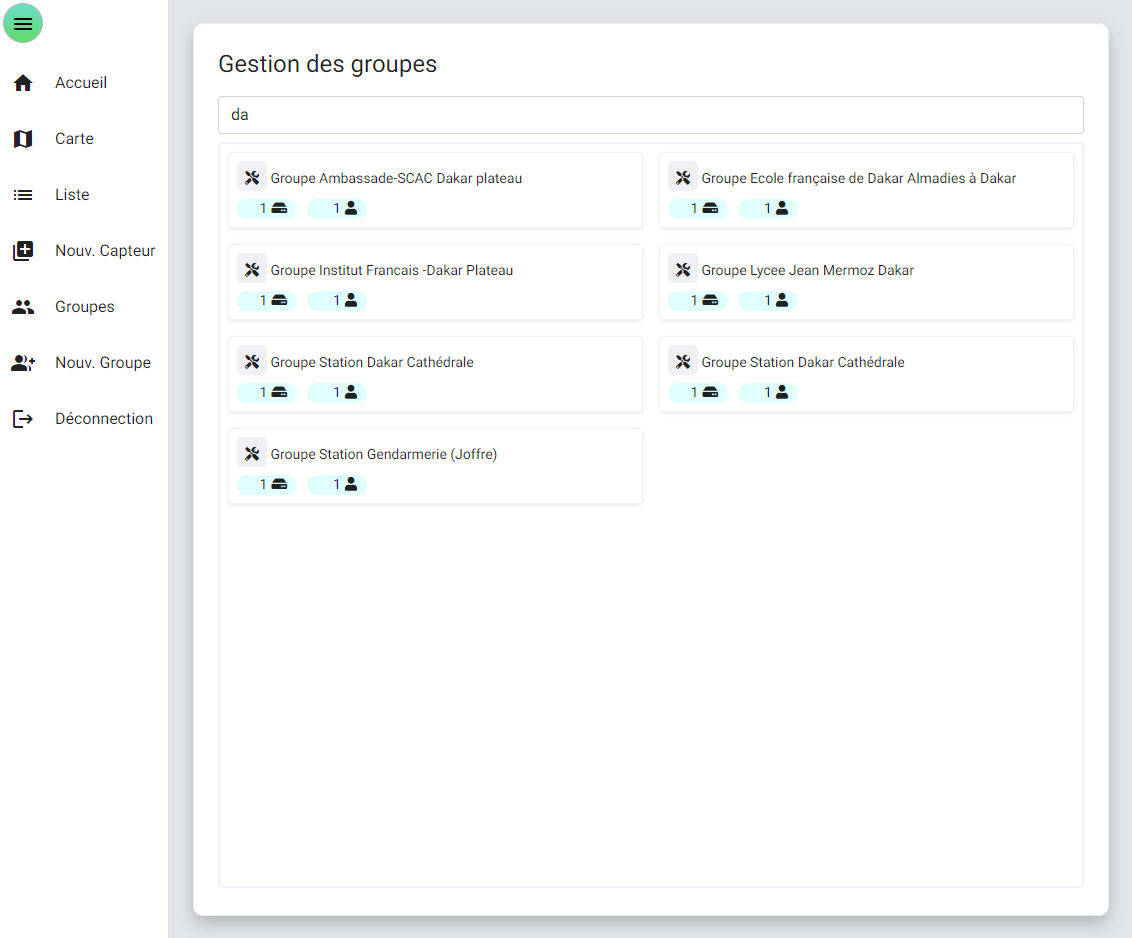
\includegraphics[width=12cm]{resources/group_search}
            \end{center}
            \caption{Rechercher un groupe}\label{fig:group-search}
        \end{figure}

        Afin de rechercher un groupe vous devez dans un premier temps être connecté et vous rendre dans l'onglet ``Groupes''.
        Vous pouvez sélectionner un groupe directement ou entrer le nom du groupe voulu dans la barre de recherche où il est indiqué ``Rechercher''.
        Une fois que vous avez clicker dessus vous retrouverez sur la page de gestion du groupe ci-dessous.


    \subsection{Gérer un groupe}\label{subsec:gerer-un-groupe}

        \begin{figure}[H]
            \begin{center}
                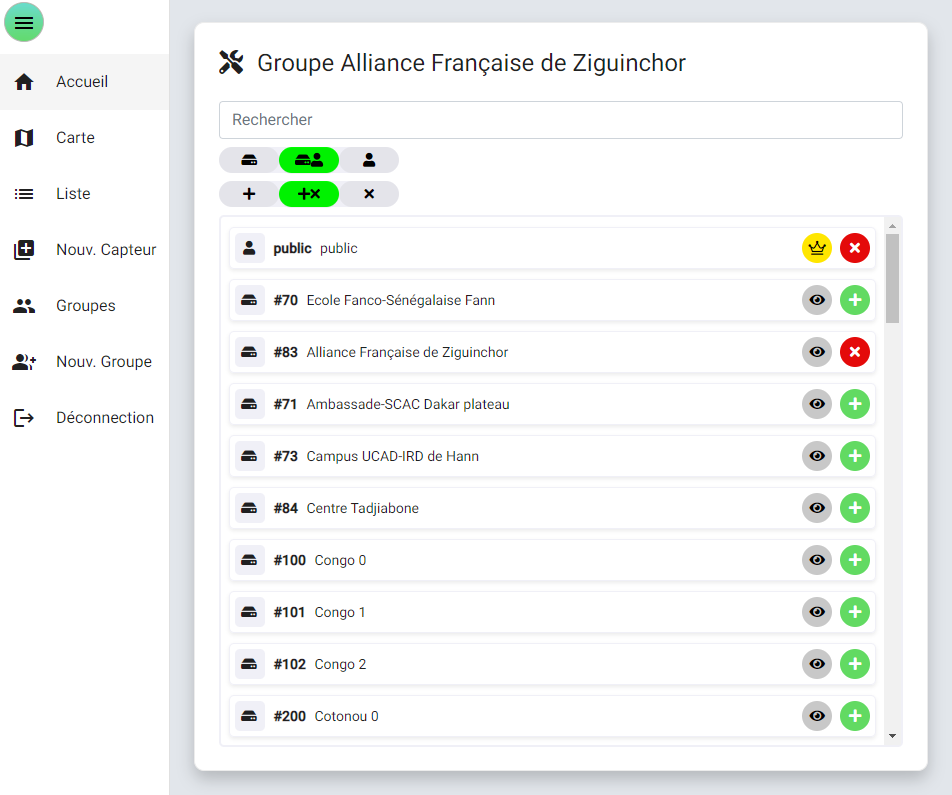
\includegraphics[width=12cm]{resources/group_manage}
            \end{center}
            \caption{Gérer un groupe}\label{fig:group-manage}
        \end{figure}

        Une fois sur cette page, vous pouvez choisir d'afficher seulement les utilisateurs, les capteurs ou les deux.
        Mais aussi choisir d'afficher les entitées (Capteur / membre) présentes dans le groupes, absent du groupe ou les deux.
        Ensuite pour chaque utilisateur vous pourrez choisir de l'ajouter au groupe ainsi que le supprimer ou le promouvoir s'il et déjà présent.
        Pour les capteurs ous pouvez accéder à leurs pages et les ajouter /supprimer du groupe.

    \section{Notification par mail}\label{sec:notification-par-mail}

    \begin{figure}[H]
        \begin{center}
            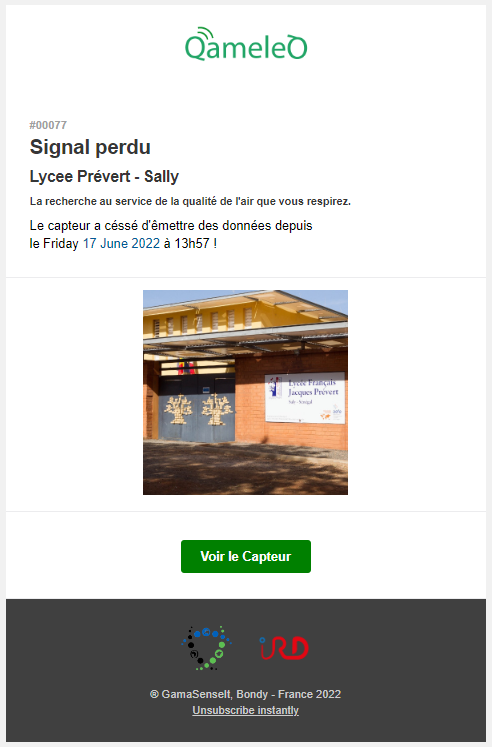
\includegraphics[width=7cm]{resources/mail}
        \end{center}
        \caption{Exemple de mail}\label{fig:exemple-de-mail}
    \end{figure}

    Le mail ci-dessous est envoyé après 24h d'absence de réception de données d'un capteur.
    Il permet d'être mis au courant rapidement des pannes.

\end{document}
